\documentclass[12pt]{paper}
\usepackage{amsmath}
\usepackage{amssymb}
\usepackage{graphicx}
\usepackage{hyperref}
\usepackage{color}
\usepackage{float}
\begin{document}
\title{Microscopic Description of DNA and Nucleusome Loss}
\maketitle
  To provide a microscopic description of nucleosome loss in the ROI, we need to state some observations and assumptions:
  \begin{enumerate}
  	\itemsep0em
  	\item histone- wrapped DNA is 3 times more probable to be damaged by UV than the linker DNA;
  	\item repair mechanism presence indicate damage site;
  	\item the repair zone is roughly circular;
  	\item the repair zone grows 3 times in area, $\sqrt{3}$ times the radius;
  	\item repair must occur on a naked DNA, with no histones on it; 
  	\item histones can be pushed any distance;
  	\item histones can slide over damage sites (since they have damages on the DNA that is wrapped around them);
  	\item length of linker DNA=50bp, length of histone-wrapped DNA=150bp;
  	\item we consider nuclesome to be the linker + the histones as a unit.   
  \end{enumerate}
     With these assumptions and observations, I present a simplified 1D model which accounts for 14\% loss of histones, with no loss of DNA, in a region expanding $\sqrt{3}$ times its initial size. 
     
     Results of simulations show that we can obtain 20\% loss of both DNA and nucleosomes due to repair protein crowding in the damage site, although this number can be increased. A total of 40\% loss of nucleosomes is seen. In this report I show that the extra percentages of loss can be attributed to nucleosome sliding, cause by exposing the damaged DNA (unwrapping it from histones) by repair proteins.
     
     The first principle to take into account is that sliding histones over any point of the DNA displaces that point 150bp left or right, depending on histone sliding direction (Figure 1). This is because one full turn of the histone is about 150bp long.This displacement is not a displacement of the point on the actual DNA, but caused by the unwinding of the DNA wrapped around the histone by rolling it.
     
     We know that the radius of the repair zone increases $\sqrt{3}$ folds. This means that the right most damage point should be translated $\sqrt{3}$ times to the right (Fig. 2). 

     If the packed region of the DNA contains $N$ nucleosomes is $L$ (Fig. 2), then to translate a point $S$, initially at $L$ to $\sqrt{3}L$, we need to displace it a distance equivalent to the total length of linker DNA in $(\sqrt{3}-1)L=0.732L$, which means $0.732N50=36.6N$ bp long. The number of times we have to slide a histone over the point $S$ is thus $36.6N/150$.
     The number $36.6N/150$ is also the number of histones transfered from the left to the right hand side of the point $S$ as it is being pushed towards $\sqrt{3}L$.
     In the region $\sqrt{3}L$ we initially have $\sqrt{3}N$ nucleosomes. After the point $S$ has reached $\sqrt{3}L$ the region contains $N-36.6N/150$ nucleosomes. 
     
     Since the point $S$ has reached $\sqrt{3}L$, and it is a damage site, we expect to find tagged repair proteins there, and by which we determine the boundary of the ROI. Thus, the percentage of histone loss from the ROI of length $\sqrt{3}$ is
     
     \begin{equation*}
     \frac{36.6N}{150\sqrt{3}N}=0.14
     \end{equation*}
     which is independent of $N$
          
     Minor adjustments to the length of the DNA wrapped around histones drives this percentage up. For instance, if instead of 1.5 turns of DNA around a histone we have only one single turn while displacing histones, then this account for 100 bp translation of damage points while rolling histones over them. Plugging this number in the denominator of the equation above gives 21\%. 
     
	\begin{figure}
	\centering
	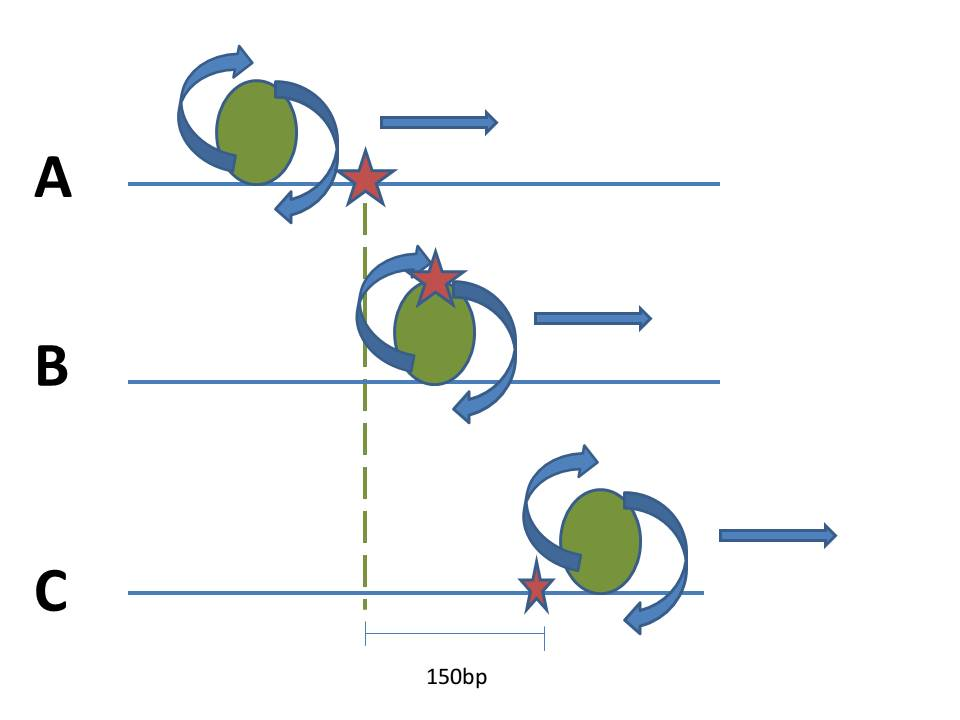
\includegraphics[width=0.7\linewidth]{histoneSlidingSingle}
	\caption{{Three time points during a displacement of damage site (red star)  causes a caused by histone rolling. The displacement of the damage site is equivalent to the length of DNA wrapped on a histone. A displacement is relative to some reference point, like the origin, and does not refer to an actual motion on the DNA}}
	\label{fig:histoneSlidingSingle}
	\end{figure}
	
	
	\begin{figure}
	\centering
	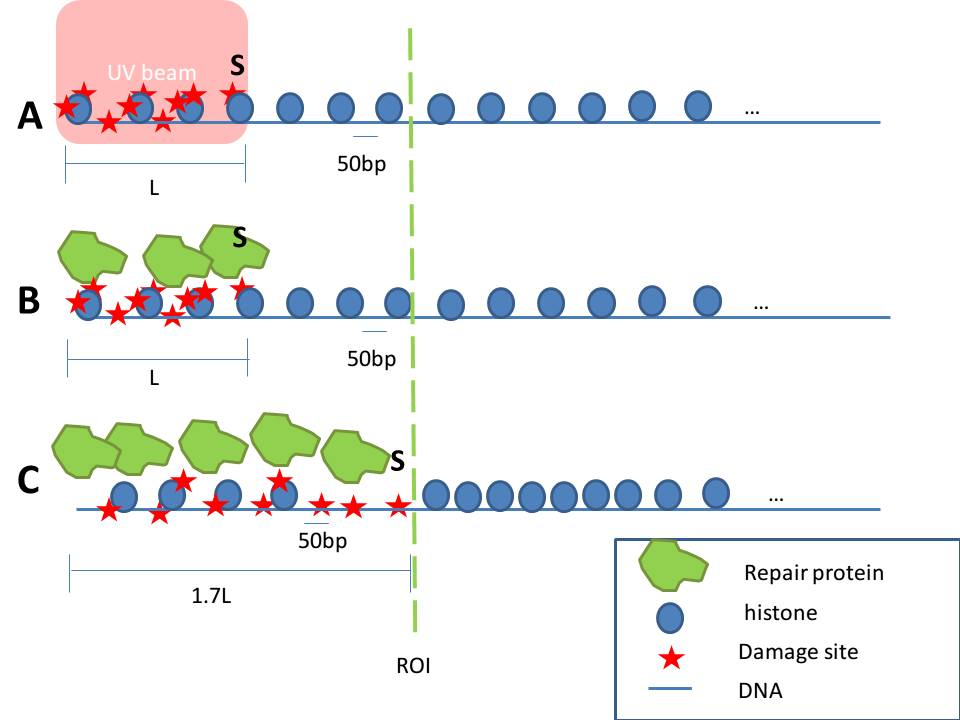
\includegraphics[width=0.7\linewidth]{histoneSlidingMulti}
	\caption{Expansion of the ROI due to nucleusome rolling. \textbf{A}. a UV beam (transparent red) damages DNA, with the point $S$ being the rightmost damage site \textbf{B}. Repair proteins (green polygons) are recruited to the damage site and start to expose the DNA in order the repair damages. \textbf{C}. Sliding the nucleosomes to the right in order to expose damage sites, translates the point $S$ to the right until $S$ reached $sqrt{3}L$. Repair proteins are present at the new location. The presence of repair proteins in $\sqrt{3}L$ indicates the ROI's boundary (vertical dashed green line)}
	\label{fig:histoneSlidingMulti}
	\end{figure}
\end{document}